\section{In-the-middle applied to max-sum problems}

\begin{figure}
	\centering
	\begin{tikzpicture}[node distance=.25cm and .25cm]
	\begin{scope}[local bounding box=components]
		% Constraint table
		\node (table) {
			\begin{tikzpicture}[scale=.8]
				\draw[step=1,black,thin] (0,0) grid (3,3);
				\node[anchor=center] at ( .5, .5) {\(-\infty\)};
				\node[anchor=center] at ( .5,1.5) {\(0\)};
				\node[anchor=center] at ( .5,2.5) {\(0\)};
				\node[anchor=center] at (1.5, .5) {\(0\)};
				\node[anchor=center] at (1.5,1.5) {\(0\)};
				\node[anchor=center] at (1.5,2.5) {\(0\)};
				\node[anchor=center] at (2.5, .5) {\(0\)};
				\node[anchor=center] at (2.5,1.5) {\(0\)};
				\node[anchor=center] at (2.5,2.5) {\(0\)};
			\end{tikzpicture}
		};
		% Upper variable
		\node[above=of table] (upper-var) {
			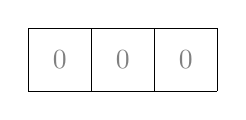
\begin{tikzpicture}[scale=.8]
				\draw[step=1,black,thin] (0,0) grid (3,1);
				\node[anchor=center] at ( .5,.5)
					{\textcolor{gray}{\(0\)}};
				\node[anchor=center] at (1.5,.5)
					{\textcolor{gray}{\(0\)}};
				\node[anchor=center] at (2.5,.5)
					{\textcolor{gray}{\(0\)}};
			\end{tikzpicture}
		};
		% Left variable
		\node[left=of table] (left-var) {
			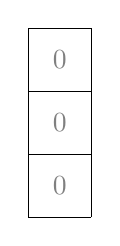
\begin{tikzpicture}[scale=.8]
				\draw[step=1,black,thin] (0,0) grid (1,3);
				\node[anchor=center] at (.5, .5)
					{\textcolor{gray}{\(0\)}};
				\node[anchor=center] at (.5,1.5)
					{\textcolor{gray}{\(0\)}};
				\node[anchor=center] at (.5,2.5)
					{\textcolor{gray}{\(0\)}};
			\end{tikzpicture}
		};
	\end{scope}
	% explanatory texts
	\node[below=of components] (cc-text) {\emph{constraint component \(g_k(x_i,x_j)\)}}
		(cc-text.east) edge[pointer,bend right=67.5] (table.east);
	\node[above=of components] (vc-text) {\emph{variable components \(x_i,x_j\)}}
		(vc-text.east) edge[pointer,bend left=67.5] (upper-var.east)
		(vc-text.west) edge[pointer,bend right=67.5] (left-var.north west);
		%\node[anchor=west] (0, .25) {\emph{constraint component}};
		%\node (2.25, 1) {}
		%	edge[pointer,bend right=22.5] (2.25,1.25) {};
		%
\end{tikzpicture}

	\caption{A single constraint of two variables \(x_i,x_j\) with \(\abs{D}=3\), and consequently a cost table \(g_k(x_i,x_j)\) with nine values. Values in the variable components are taken from \(\bar{c}\) ,values in the constraint component are properties of the problem.}
\end{figure}


\begin{figure}
	\centering
	\subfloat[Initial constraint]{\input{figs/cost-function-update-1.tikz}}
	\hfil
	\subfloat[The \enquote{move in} operation]{\input{figs/cost-function-update-2.tikz}}
	\hfil
	\subfloat[The \enquote{move out} operation]{\input{figs/cost-function-update-3.tikz}}
	\caption{An illustration of a single fractional DP update with \(\alpha = n^{-1} = \num{0.5}\).}
\end{figure}

\begin{algorithm}[tbp]
	\Repeat{no sign changes in \(\bar{c}\)}{
		\ForAll{cost functions \(g_k\)}{
			\ForAll{\(w^k : g_k(w^k) > -\infty\)}{
				
			}
		}
	}

	\caption{The max-sum in-the-middle algorithm (\emph{c.f.} \cref{alg:itm-lp-heur}).}
	\label{alg:itm-max-sum}
\end{algorithm}

\subsection{Improvements}


\subsubsection{The \enquote{push} operation}
In their asessment of the in-the-middle algorithm, \textcite{Bastert10} introduce a number of generalizations and improvements.
One of these improvements is the so-called \enquote{push} operation.
The idea of the push operation is to guide the algorithm toward better solutions after a first feasible solution is found.

Since the algorithm with its heuristic is approximative, any feasible solution found is only guaranteed to be optimal for \(\bar{c}\), \emph{i.e.} the modified cost vector.
\Citeauthor{Bastert10} define the \enquote{push} operation \parencite[\pno~100]{Bastert10} as setting \(\bar{c} \leftarrow \bar{c} + \rho c\) for some parameter \(\rho\) whenever a feasible solution is found, then continuing to run the algorithm for at least 50 iterations.
Additionally, the parameter \(\kappa\) used in the algorithm is reduced by a factor in the push operation.

The push operation is in essence a local search.
When a feasible solution to the approximative problem (as generated by the heuristic) is found, that solution is used as a starting point for a less aggressive heuristic or the exact algorithm on the original problem.

For max-sum problems, the original vector \(c\) will always be all-zero.
Therefore, the push operation is implemented as setting \(\bar{c} \leftarrow c\), which is roughly equivalent to \(\rho=\infty\).
The parameter \(\kappa\) is multiplied by a factor \num{0.8}.

\subsubsection{The cost function reset operation}
% [todo] - more formal motivation with the language of Wedelin08/13
Building on the idea behind the \enquote{push} operation, which is less meaningful in the max-sum case where the reduced cost vector \(\bar{c}\) only implicitly defines the costs, one may define a similar operation that instead applies directly to the cost functions \(g_k\).
The general idea is similar; every iteration changes the cost functions \(g_k\) and for sufficiently large \(\kappa\) that operation is \emph{conflicting} \parencite[\pno~15\psq]{Wedelin13} which means the algorithm may converge to non-global optima.

By resetting the cost functions \(g_k\) to their original value while keeping the current \(\bar{c}\) (which implicitly defines the \enquote{current} solution), we may hope to return the problem to its original form and perhaps find better solutions.
% [review] - notation for vector s?
In addition to resetting \(g_k\), the operation also sets \(s_i=0\) for all constraints, effectively making them forget any changes they have made to \(\bar{c}\).
After performing a cost function reset, the \(\kappa\) parameter is multiplied by \num{0.8} and the algorithm continues for at least 50 more iterations.


\subsection{Interpretations in other fields}
